\documentclass[14pt]{extbook}
\usepackage{multicol, enumerate, enumitem, hyperref, color, soul, setspace, parskip, fancyhdr} %General Packages
\usepackage{amssymb, amsthm, amsmath, bbm, latexsym, units, mathtools} %Math Packages
\everymath{\displaystyle} %All math in Display Style
% Packages with additional options
\usepackage[headsep=0.5cm,headheight=12pt, left=1 in,right= 1 in,top= 1 in,bottom= 1 in]{geometry}
\usepackage[usenames,dvipsnames]{xcolor}
\usepackage{dashrule}  % Package to use the command below to create lines between items
\newcommand{\litem}[1]{\item#1\hspace*{-1cm}\rule{\textwidth}{0.4pt}}
\pagestyle{fancy}
\lhead{Makeup Progress Quiz 1}
\chead{}
\rhead{Version B}
\lfoot{6018-3080}
\cfoot{}
\rfoot{Spring 2021}
\begin{document}

\begin{enumerate}
\litem{
Construct the lowest-degree polynomial given the zeros below. Then, choose the intervals that contain the coefficients of the polynomial in the form $ax^3+bx^2+cx+d$.\[ \frac{-3}{2}, \frac{-6}{5}, \text{ and } \frac{7}{4} \]\begin{enumerate}[label=\Alph*.]
\item \( a \in [40, 41], b \in [37, 46], c \in [-118, -115], \text{ and } d \in [-127, -124] \)
\item \( a \in [40, 41], b \in [-178, -176], c \in [250, 263], \text{ and } d \in [-127, -124] \)
\item \( a \in [40, 41], b \in [37, 46], c \in [-118, -115], \text{ and } d \in [126, 127] \)
\item \( a \in [40, 41], b \in [-47, -32], c \in [-118, -115], \text{ and } d \in [126, 127] \)
\item \( a \in [40, 41], b \in [-82, -80], c \in [-56, -48], \text{ and } d \in [126, 127] \)

\end{enumerate} }
\litem{
Describe the end behavior of the polynomial below.\[ f(x) = 6(x - 5)^{4}(x + 5)^{7}(x + 9)^{3}(x - 9)^{5} \]\begin{enumerate}[label=\Alph*.]
\begin{multicols}{2}\item 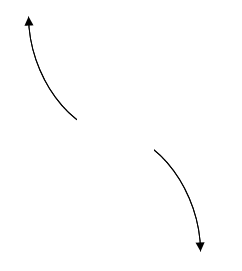
\includegraphics[width = 0.3\textwidth]{../Figures/polyEndBehaviorAB.png}\item 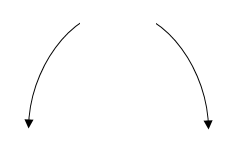
\includegraphics[width = 0.3\textwidth]{../Figures/polyEndBehaviorBB.png}\item 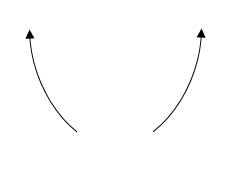
\includegraphics[width = 0.3\textwidth]{../Figures/polyEndBehaviorCB.png}\item 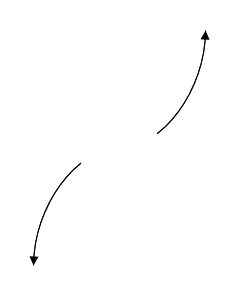
\includegraphics[width = 0.3\textwidth]{../Figures/polyEndBehaviorDB.png}\end{multicols}\item None of the above.
\end{enumerate} }
\litem{
Construct the lowest-degree polynomial given the zeros below. Then, choose the intervals that contain the coefficients of the polynomial in the form $x^3+bx^2+cx+d$.\[ -2 + 2 i \text{ and } 3 \]\begin{enumerate}[label=\Alph*.]
\item \( b \in [0, 1.7], c \in [-4.1, -3.6], \text{ and } d \in [-27, -20] \)
\item \( b \in [-3.8, 0.8], c \in [-4.1, -3.6], \text{ and } d \in [21, 27] \)
\item \( b \in [0, 1.7], c \in [-5.5, -4.1], \text{ and } d \in [6, 7] \)
\item \( b \in [0, 1.7], c \in [-3.9, 3.7], \text{ and } d \in [-9, -3] \)
\item \( \text{None of the above.} \)

\end{enumerate} }
\litem{
Construct the lowest-degree polynomial given the zeros below. Then, choose the intervals that contain the coefficients of the polynomial in the form $ax^3+bx^2+cx+d$.\[ \frac{7}{4}, \frac{1}{4}, \text{ and } \frac{2}{3} \]\begin{enumerate}[label=\Alph*.]
\item \( a \in [44, 56], b \in [126, 137], c \in [81, 90], \text{ and } d \in [11, 17] \)
\item \( a \in [44, 56], b \in [-135, -118], c \in [81, 90], \text{ and } d \in [11, 17] \)
\item \( a \in [44, 56], b \in [63, 68], c \in [-46, -41], \text{ and } d \in [-14, -7] \)
\item \( a \in [44, 56], b \in [-135, -118], c \in [81, 90], \text{ and } d \in [-14, -7] \)
\item \( a \in [44, 56], b \in [39, 42], c \in [-69, -65], \text{ and } d \in [11, 17] \)

\end{enumerate} }
\litem{
Construct the lowest-degree polynomial given the zeros below. Then, choose the intervals that contain the coefficients of the polynomial in the form $x^3+bx^2+cx+d$.\[ 2 - 3 i \text{ and } -2 \]\begin{enumerate}[label=\Alph*.]
\item \( b \in [0.54, 1.9], c \in [-1, 4], \text{ and } d \in [-4, -2] \)
\item \( b \in [1.49, 3.68], c \in [5, 7], \text{ and } d \in [-31, -17] \)
\item \( b \in [0.54, 1.9], c \in [5, 7], \text{ and } d \in [4, 8] \)
\item \( b \in [-2.47, -1.16], c \in [5, 7], \text{ and } d \in [19, 30] \)
\item \( \text{None of the above.} \)

\end{enumerate} }
\litem{
Which of the following equations \textit{could} be of the graph presented below?
\begin{center}
    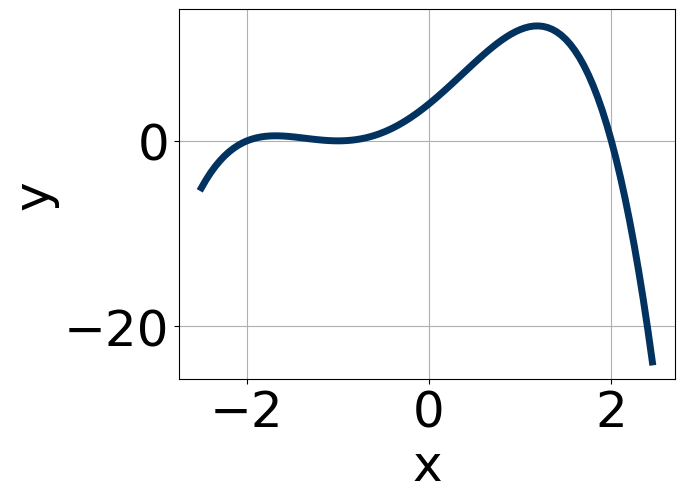
\includegraphics[width=0.5\textwidth]{../Figures/polyGraphToFunctionB.png}
\end{center}
\begin{enumerate}[label=\Alph*.]
\item \( -11(x + 1)^{10} (x + 2)^{10} (x - 2)^{7} \)
\item \( -9(x + 1)^{6} (x + 2)^{11} (x - 2)^{5} \)
\item \( 4(x + 1)^{8} (x + 2)^{5} (x - 2)^{9} \)
\item \( -14(x + 1)^{5} (x + 2)^{6} (x - 2)^{5} \)
\item \( 10(x + 1)^{8} (x + 2)^{11} (x - 2)^{8} \)

\end{enumerate} }
\litem{
Describe the zero behavior of the zero $x = 7$ of the polynomial below.\[ f(x) = 5(x + 5)^{12}(x - 5)^{8}(x - 7)^{10}(x + 7)^{5} \]\begin{enumerate}[label=\Alph*.]
\begin{multicols}{2}\item 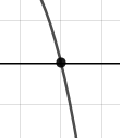
\includegraphics[width = 0.3\textwidth]{../Figures/polyZeroBehaviorCopyAB.png}\item 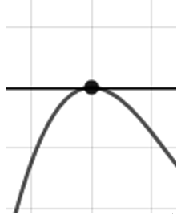
\includegraphics[width = 0.3\textwidth]{../Figures/polyZeroBehaviorCopyBB.png}\item 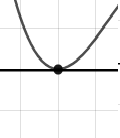
\includegraphics[width = 0.3\textwidth]{../Figures/polyZeroBehaviorCopyCB.png}\item 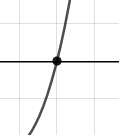
\includegraphics[width = 0.3\textwidth]{../Figures/polyZeroBehaviorCopyDB.png}\end{multicols}\item None of the above.
\end{enumerate} }
\litem{
Describe the end behavior of the polynomial below.\[ f(x) = -8(x + 7)^{2}(x - 7)^{3}(x + 5)^{2}(x - 5)^{3} \]\begin{enumerate}[label=\Alph*.]
\begin{multicols}{2}\item 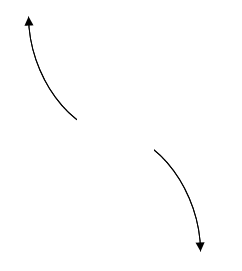
\includegraphics[width = 0.3\textwidth]{../Figures/polyEndBehaviorCopyAB.png}\item 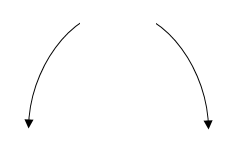
\includegraphics[width = 0.3\textwidth]{../Figures/polyEndBehaviorCopyBB.png}\item 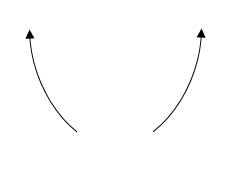
\includegraphics[width = 0.3\textwidth]{../Figures/polyEndBehaviorCopyCB.png}\item 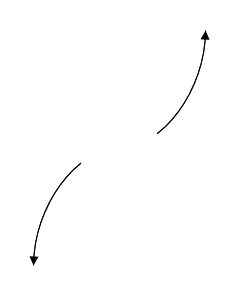
\includegraphics[width = 0.3\textwidth]{../Figures/polyEndBehaviorCopyDB.png}\end{multicols}\item None of the above.
\end{enumerate} }
\litem{
Which of the following equations \textit{could} be of the graph presented below?
\begin{center}
    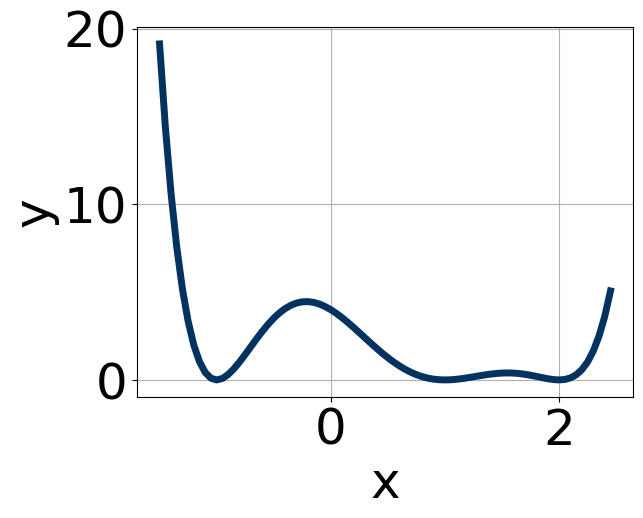
\includegraphics[width=0.5\textwidth]{../Figures/polyGraphToFunctionCopyB.png}
\end{center}
\begin{enumerate}[label=\Alph*.]
\item \( 14(x - 2)^{8} (x - 1)^{7} (x + 1)^{5} \)
\item \( 12(x - 2)^{4} (x - 1)^{10} (x + 1)^{9} \)
\item \( -3(x - 2)^{6} (x - 1)^{10} (x + 1)^{8} \)
\item \( 2(x - 2)^{4} (x - 1)^{4} (x + 1)^{6} \)
\item \( -6(x - 2)^{10} (x - 1)^{4} (x + 1)^{9} \)

\end{enumerate} }
\litem{
Describe the zero behavior of the zero $x = 8$ of the polynomial below.\[ f(x) = -5(x + 3)^{7}(x - 3)^{5}(x + 8)^{6}(x - 8)^{3} \]\begin{enumerate}[label=\Alph*.]
\begin{multicols}{2}\item 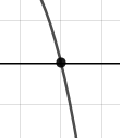
\includegraphics[width = 0.3\textwidth]{../Figures/polyZeroBehaviorAB.png}\item 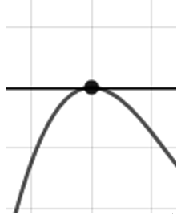
\includegraphics[width = 0.3\textwidth]{../Figures/polyZeroBehaviorBB.png}\item 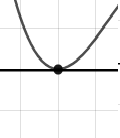
\includegraphics[width = 0.3\textwidth]{../Figures/polyZeroBehaviorCB.png}\item 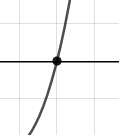
\includegraphics[width = 0.3\textwidth]{../Figures/polyZeroBehaviorDB.png}\end{multicols}\item None of the above.
\end{enumerate} }
\end{enumerate}

\end{document}